%!TEX root = ../icip_jseo.tex
% -*- root: ../icip_jseo.tex -*-


\section{Experiments}

% 앞에서 제안한 특징점 Filtering 알고리즘을 이용하여 학습을 수행하였을 때 인식 성능의 개선을 측정하였다. 

% 실험 영상은, 서울시 가이드 지도 팜플릿 영상 16장을 선택하여 사용되었다. 이러한 영상을 rotation($0.5\sim2.0$배, 0.1배 간격), scale($0\degree\sim360\degree$, $10\degree$ 간격), blur(Gaussian blur, $r=0,3,5,7$pixels) 등의 변형(deformed)한 영상 32,256장 중 random sampling하여 train images 16,114장, test images 16,142장을 선택하였다.
% 먼저 train images에서 특징점들을 검출(detect)하고, detected keypoint 들을 이용하여 앞의 정의된 Score function($gf(p_i)$)을 계산하였다. 

The improvement of recognition performance after the training using the keypoints filtering algorithm proposed earlier was measured. As for the experimental images, 16 images of Seoul Guide Map Pamphlet was selected. These images were deformed by way of rotating($0.5\sim2.0$-folds, at the interval of 0.1-fold) scaling (($0\degree\sim360\degree$, at the interval of $10\degree$ intervals) and blurring (Gaussian blur, $r = 0,3,5,7$ pixels). As a result, 32,256 images were obtained. Of them, 16,114 training images and 16,142 test images were selected at random. First, the keypoints of training images were detected and then the score function($gf(p_i)$) was calculated using the detected keypoints. 


%특징점 데이터베이스는 Score function을 고려하지 않은 전체 특징점 집합($K_{all}, n(K_{all}) = 3000$)과, Score function에서 상위 50개, 100개, 300개, 500개 특징점들만 filtering 하여 구성한 특징점 집합($K_{50}, K_{100}, K_{300}, K_{500}$)으로 구성되었다. 
The keypoints database is composed of the set of all keypoints($K_{all}, n(K_{all}) = 3000$) that did not consider the score function and the set of the keypoints($K_{50}, K_{100}, K_{300}, K_{500}$) composed of top 50, 100, 300 and 500 keypoints filtered in the score function. 


%먼저 인식 속도 향상 정도를 측정하였다. 제안하는 방법은 train 단계에서 특징점들을 줄여 저장하기 때문에 비교 대상이 되는 특징점들의 개수가 줄어들게 된다. 이에 따라 연산의 속도가 향상되게 된다.
First the improvement of recognition speed was measured. As for the proposed method, since the keypoints were reduced to be saved in the training phase, the number of the keypoints, the subjects of comparison, decreases, which in turn increases the computing speed. 

\begin{figure}[ht!]
\centering
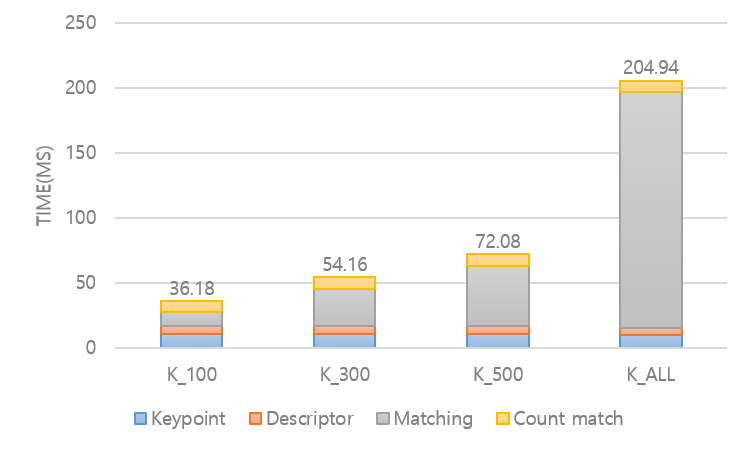
\includegraphics[width=1.0\columnwidth]{4_experiments/ex_time}
\caption{Time Comparison Among Conventional Full Database and Proposed Filtered Database}
\label{fig:markerless_time_experiments}
\end{figure}

\label{fig:markerless_speed}
% 그림 \ref{fig:markerless_speed}에서 보듯이 연산 속도는 특징점 집합의 개수에 따라서 비례하여 향상되고 있다. 특히, 100개로 학습한 경우에서는 전체 특징점을 학습한 경우에 비하여 소요 시간이 $1/n$으로 감소됨을 볼 수 있다. Smart phone과 같이 경량화 된 실행 환경에서는 이렇게 연산량을 줄여줌으로써 빠른 interaction을 제공할 수 있게 된다.

%제안하는 방법은 속도를 향상시키면서도 전체적인 인식성능의 향상도 기대할 수 있다. 이러한 특징점 데이터베이스를 이용하여 test images와의 인식 성능을 측정하였다. 인식 성능 측정을 위한 Match 방법은 \cite{choi_smart_2014}의 방법을 사용하여 false match를 최대한 억제하는 match 방법을 적용하였다.

As shown in Figure \ref{fig:markerless_speed}, the computing speed improves in proportion to the number of the set of keypoints. In particular, the time spent for training deceases to $1/n$ compared to the training of whole keypoints when training was performed with 100 keypoints. In a lightweight implementation environment like smartphone, the reduction of computation provides rapid interaction. The proposed method is expeted to increases the speed and to improve the overall recognition performance. The test image recognition performance was measured using keypoints database. As for the match method for measuring recognition performance, we used the match method\cite{choi_smart_2014} which suppressing the false match to the max. 

% 이를 이용하여 인식율을 측정한 결과는 그림 \ref{fig:markerless_roc}와 같다. 전체 특징점 집합($K_{all}$)을 사용한 특징점 데이터베이스와 비교하여, $K_{500}$과 $K_{300}$은 조금 인식율의 저하가 보여졌으나, $K_{100}$과 $K_{50}$은 성능이 향상되었다. 

The results of the measurement of recognition rate using the above method were demonstrated in Figure \ref{fig:markerless_roc}. In comparison with the keypoints database using the whole of keypoint sets($K_{all}$), $K_{500}$ and $K_{300}$ showed slight degradation of recognition rate whereas $K_{100}$ and $K_{50}$ showed the improvement of performance.  

%%%%%분석 결과가 더 들어가면 좋겠다%%%%%


\begin{figure}[ht!]
\centering
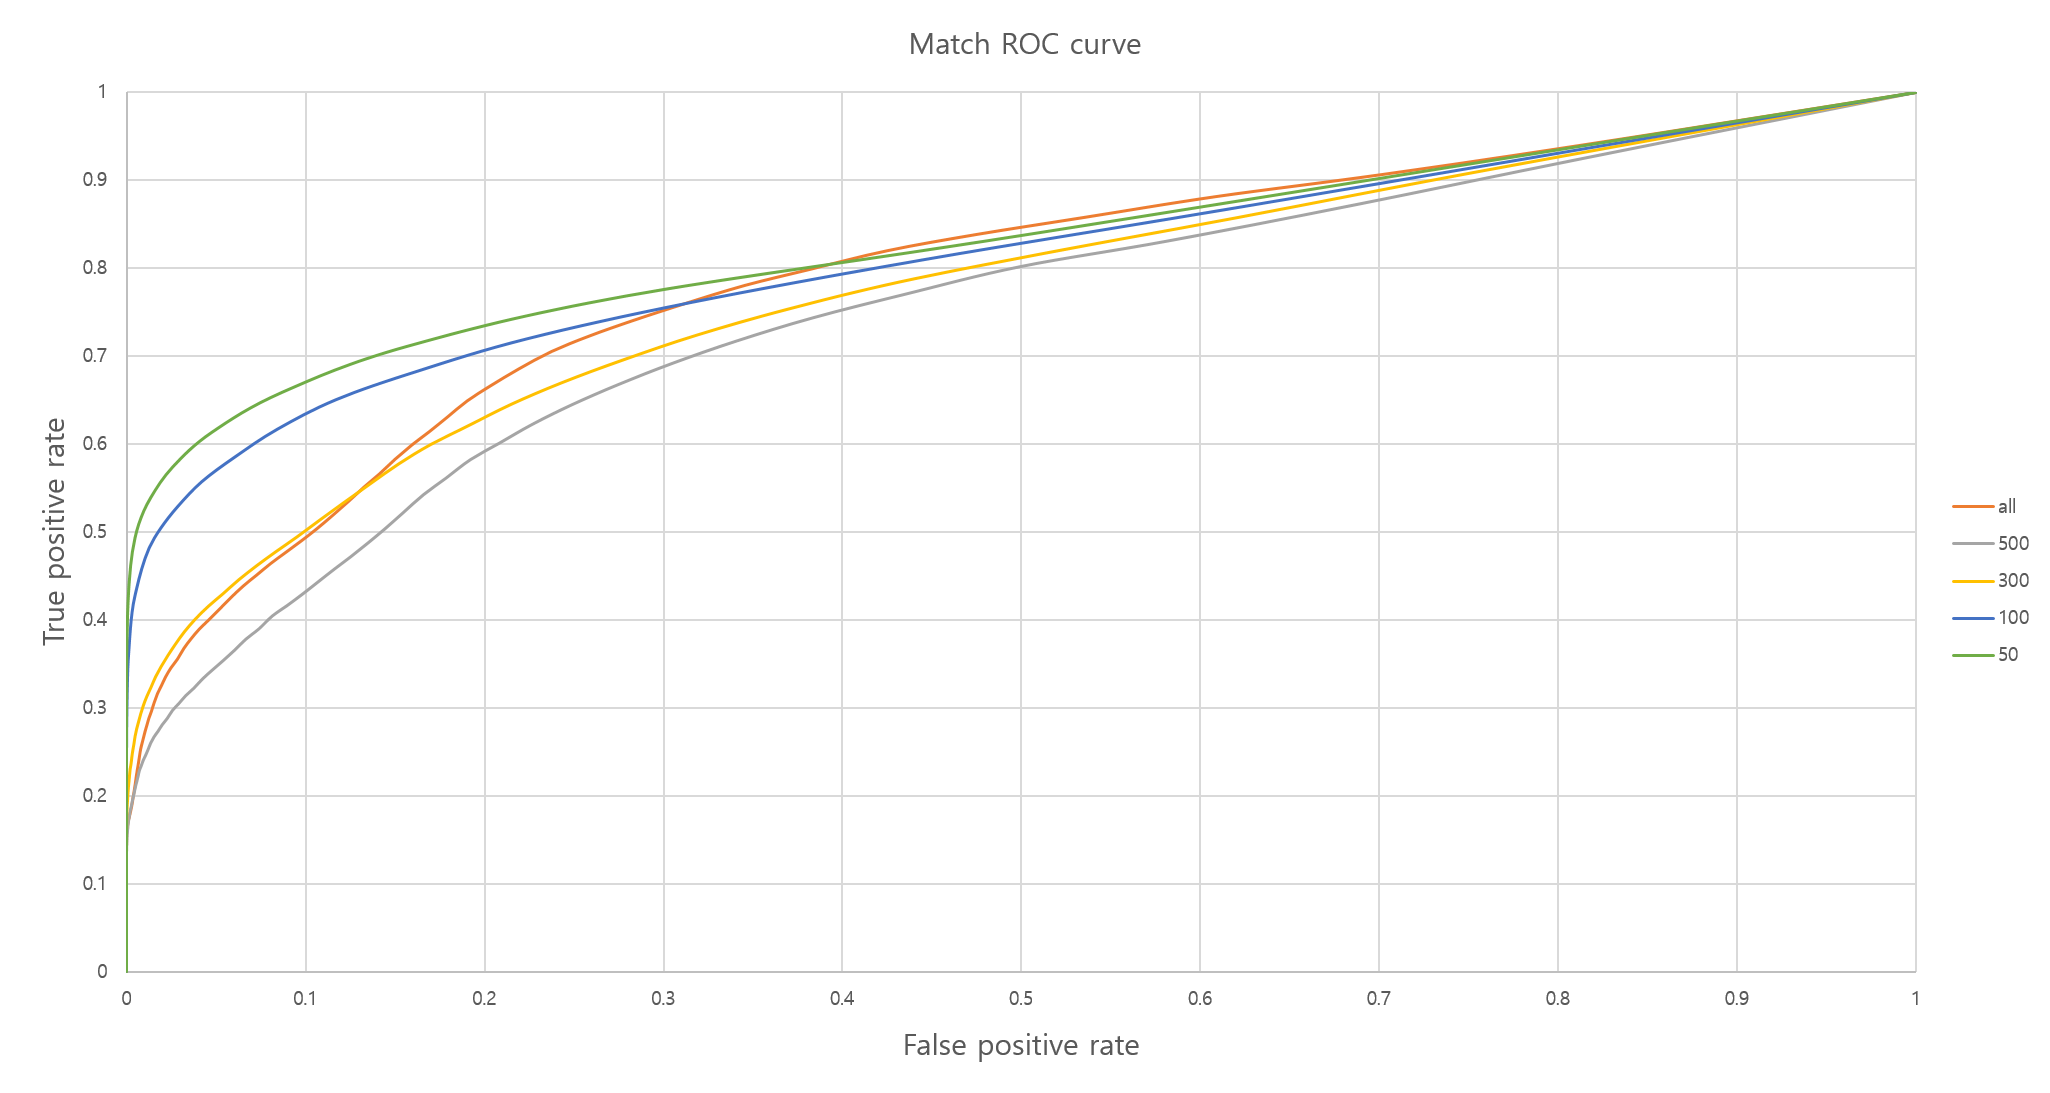
\includegraphics[width=1.0\columnwidth]{4_experiments/roc}
\caption{ROC curve for match rate}
\label{fig:markerless_roc}
\end{figure}

% 이러한 keypoint filtering을 수행하게 되면, miss-match를 유발하는 bad keypoint가 제거되기 때문에 match 결과의 reliability 가 높아진다. 이를 증명하기 위하여 Feature-level에서 Precision\cite{heinly_comparative_2012}을 계산하였다. Precision은 match 결과 구해진 correspondence pair의 수 대비 correct match의 비율로 계산이 된다. 이는 match 결과에 얼마나 miss-match가 적고 correct match의 비율이 높은지를 나타낸다. match 결과 대비 correct match의 비율이 높을수록 이후에 robust pose estimation의 성능에 영향을 미친다.

When performing keypoint filtering, the bad keypoints causing miss-match are eliminated, which in turn increases the reliability of the match results. To prove this, the precision\cite{heinly_comparative_2012} in the feature-level was calculated. The precision can be calculated as the ratio between the number of the correspondence pairs obtained after matching and the correct matches, indicating the insignificant proportion of mass-match and significant proportion of correction match in the match results. The increase of the ratio between correct match and match results subsequently affects the performance of robust pose estimation. 


\begin{figure}[t!]
\centering
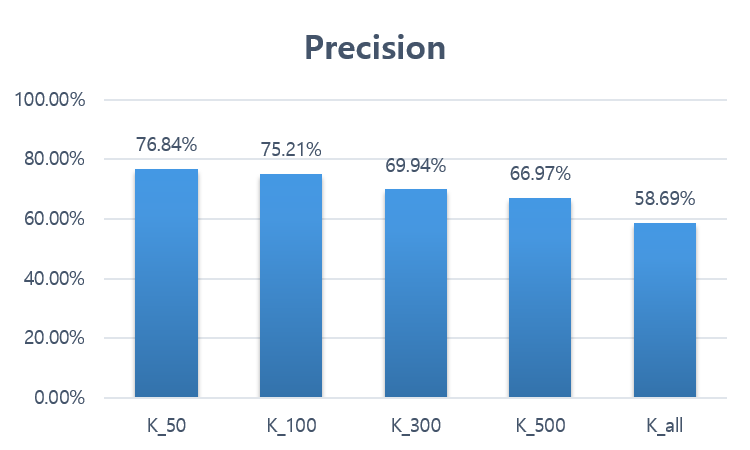
\includegraphics[width=1.0\columnwidth]{4_experiments/precision}
\caption{Precision of filtered keypoint database}
\label{fig:markerless_precision}
\end{figure}

\begin{table}[b!]
\centering
%\resizebox{\columnwidth}{!}{%
\begin{tabular}{llllll}
\hline
\textbf{}                   & \textbf{$K_{50}$} & \textbf{$K_{100}$} & \textbf{$K_{300}$} & \textbf{$K_{500}$} & \textbf{$K_{all}$} \\
\textbf{Avg. Match Result}  & 10.098            & 15.618             & 26.747             & 31.409             & 44.859             \\
\textbf{Avg. Correct Match} & 7.759             & 11.747             & 18.705             & 21.033             & 26.326             \\
\textbf{Precision}          & 76.8\%            & 75.2\%             & 69.9\%             & 67.0\%             & 58.7\%             \\ \hline
\end{tabular}
%}
  \caption{Precision of Filtered Matching}
  \label{tab:markerless_precision}
\end{table}

% Precision의 결과는 그림 \ref{fig:markerless_precision}와 표\ref{tab:markerless_precision}에 나타난다. 전체 특징점 집합($K_{all}$)에 비하여 filtered 특징점 집합들이 더 높은 precision을 나타내주었다. 검출되는 특징점의 개수는 줄어들지만, Correct Match의 비율이 높아지기 때문에 높은 Precision을 보여주었다. 이러한 결과는 robst pose estimation의 속도와 성능을 향상시킬 수 있다.

The results of precision are demonstrated in Table \ref{tab:markerless_precision} and Table \ref{fig:markerless_precision}. The filtered keypoints sets showed higher precision compared to the whole of keypoints set ($K_{all}$). The number of the detected keypoints decreased but the ratio of correct match increased, which showed high precision. Such results are able to improve the speed and performance of robust pose estimation.  
